\documentclass{beamer}

\usepackage[russian]{babel}
\usepackage[utf8]{inputenc}
\usepackage{cmap}
\usepackage{graphicx}
\usepackage{xspace}
\usepackage{psfrag}
\usepackage{hyperref}
\usepackage[normalem]{ulem}
\usepackage{tabularx}
\usepackage{booktabs}

\beamertemplatenavigationsymbolsempty
\setbeamertemplate{footline}[frame number]
\usecolortheme{seahorse}
\setbeamerfont{footnote}{size=\tiny}

%%Исправляем греческие буквы в формулах, они должны быть прямыми, а не курсивными
\DeclareSymbolFont{greek}{U}{eur}{m}{n}                                                        
\SetSymbolFont{greek}{bold}{U}{eur}{b}{n}                                                      
\DeclareSymbolFontAlphabet{\gr}{greek}                                                         
\DeclareMathSymbol{\alpha}{\mathord}{greek}{"0B}                                               
\DeclareMathSymbol{\beta}{\mathord}{greek}{"0C}                                                
\DeclareMathSymbol{\gamma}{\mathord}{greek}{"0D}                                               
\DeclareMathSymbol{\delta}{\mathord}{greek}{"0E}                                               
\DeclareMathSymbol{\epsilon}{\mathord}{greek}{"0F}                                             
\DeclareMathSymbol{\zeta}{\mathord}{greek}{"10}                                                
\DeclareMathSymbol{\eta}{\mathord}{greek}{"11}                                                 
\DeclareMathSymbol{\theta}{\mathord}{greek}{"12}                                               
\DeclareMathSymbol{\iota}{\mathord}{greek}{"13}                                                
\DeclareMathSymbol{\kappa}{\mathord}{greek}{"14}                                               
\DeclareMathSymbol{\lambda}{\mathord}{greek}{"15}                                              
\DeclareMathSymbol{\mu}{\mathord}{greek}{"16}                                                  
\DeclareMathSymbol{\nu}{\mathord}{greek}{"17}                                                  
\DeclareMathSymbol{\xi}{\mathord}{greek}{"18}                                                  
\DeclareMathSymbol{\pi}{\mathord}{greek}{"19}                                                  
\DeclareMathSymbol{\rho}{\mathord}{greek}{"1A}                                                 
\DeclareMathSymbol{\sigma}{\mathord}{greek}{"1B}                                               
\DeclareMathSymbol{\tau}{\mathord}{greek}{"1C}                                                 
\DeclareMathSymbol{\upsilon}{\mathord}{greek}{"1D}                                             
\DeclareMathSymbol{\phi}{\mathord}{greek}{"1E}                                                 
\DeclareMathSymbol{\chi}{\mathord}{greek}{"1F}                                                 
\DeclareMathSymbol{\psi}{\mathord}{greek}{"20}                                                 
\DeclareMathSymbol{\omega}{\mathord}{greek}{"21}                                               
\DeclareMathSymbol{\varepsilon}{\mathord}{greek}{"22}                                          
\DeclareMathSymbol{\vartheta}{\mathord}{greek}{"23}                                            
\DeclareMathSymbol{\varpi}{\mathord}{greek}{"24}                                               
\let\varrho\rho                                                                                
\let\varsigma\sigma                                                                            
\DeclareMathSymbol{\varphi}{\mathord}{greek}{"27}

\title{Разработка нейросетевой модели преобразования изображения геометрических фигур в~JSON-описание}
\author[Кошелев Е.\,Ф.]{Кошелев Егор Федорович, 932302 \\ \vspace{0.5em} {\small Научный руководитель: канд.~техн.~наук, доцент \\ Михаил Сергеевич Пожидаев}}
\date{\today}

\begin{document}
\maketitle

\begin{frame}
\frametitle{Введение и актуальность}
\framesubtitle{Задача структуризации визуальной информации}
\begin{itemize}
  \item Множество прикладных задач требует перевода растрового изображения в~\textbf{структурированное машиночитаемое описание} (векторизация, распознавание схем, диаграмм, чертежей).
  \item Классические алгоритмы (поиск контуров, аппроксимация) хрупки к~перекрытиям фигур, шуму и~вариативности форм.
  \item \textbf{Идея:} рассматривать задачу как \emph{image-to-sequence} --- сквозное (end-to-end) обучение нейросети, порождающей готовый JSON.
  \item Модельный полигон: изображения с~прямоугольниками, эллипсами и~треугольниками произвольного цвета.
\end{itemize}
\end{frame}

\begin{frame}
\frametitle{Цель и задачи}
\framesubtitle{Что требуется сделать}
\textbf{Цель:} построить нейросетевую модель, преобразующую RGB-изображение геометрических фигур в~корректное JSON-описание сцены.

\medskip
\textbf{Задачи:}
\begin{enumerate}
  \item Сформировать синтетический датасет «изображение~$\to$~JSON».
  \item Спроектировать архитектуру кодер-декодер на~базе трансформера.
  \item Обучить модель в~режиме максимизации правдоподобия (MLE).
  \item Дообучить модель методом обучения с~подкреплением (RL).
  \item Оценить качество по~метрикам детекции и~геометрической близости.
\end{enumerate}
\end{frame}

\begin{frame}[fragile,shrink=8]
\frametitle{Постановка задачи}
\framesubtitle{Вход и выход модели}
\begin{columns}[T]
\begin{column}{0.62\textwidth}
\textbf{Вход:} RGB-изображение $H\times W$ (до~$512\times512$), от~1 до~10 фигур.

\smallskip
\textbf{Выход:} строка JSON\footnote{\textbf{JSON} (JavaScript Object Notation) --- текстовый формат представления структурированных данных в~виде пар ключ--значение и~массивов.} --- список объектов. Каждый объект задаёт тип фигуры~\texttt{t}, цвет~\texttt{c} и~геометрию (\texttt{bb}~--- bounding box либо \texttt{pts}~--- вершины):
\begin{verbatim}
[{"t":"ellipse","c":"#71381c",
  "bb":[7,64,137,89]},
 {"t":"triangle","c":"#ff001c",
  "pts":[220,396,228,436,250,383]}]
\end{verbatim}
\end{column}
\begin{column}{0.35\textwidth}
\centering
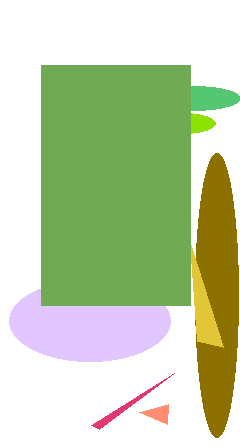
\includegraphics[width=\columnwidth,keepaspectratio]{example}\\[0.3em]
\end{column}
\end{columns}
\end{frame}

\begin{frame}
\frametitle{Синтетический датасет}
\framesubtitle{Генерация пар «изображение~--~JSON»}
\begin{itemize}
  \item $\sim$\textbf{100\,000} примеров, генерируемых процедурно (PIL).
  \item Случайные размеры холста, тип, цвет и~положение фигур (палитра из~$10^3$ цветов).
  \item \textbf{Контроль видимости:} фигуры рисуются на~маске уникальными ID; объекты, перекрытые сверху и~занимающие $<100$~пикселей, исключаются из~разметки.
  \item Треугольники проверяются на~вырожденность по~формуле площади Гаусса.
  \item Гарантия: JSON описывает только \emph{реально видимые} фигуры $\Rightarrow$ согласованность входа и~цели.
\end{itemize}
\end{frame}

\begin{frame}
\frametitle{Архитектура модели}
\framesubtitle{Кодер-декодер на~базе трансформера (image-to-sequence)}
\begin{columns}
\begin{column}{0.5\textwidth}
\textbf{Кодер изображения (ViT\footnotemark-подобный):}
\begin{itemize}
  \item Разбиение на~патчи $16\times16$.
  \item Линейная проекция в~$d=512$.
  \item Обучаемое 2D-позиционное кодирование.
  \item $6$ слоёв \texttt{TransformerEncoder}.
\end{itemize}
\end{column}
\begin{column}{0.5\textwidth}
\textbf{Декодер текста (JSON):}
\begin{itemize}
  \item Посимвольный токенайзер.
  \item 1D-позиционное кодирование.
  \item $6$ слоёв \texttt{TransformerDecoder} с~cross-attention\footnotemark\ к~патчам.
  \item Авторегрессионная генерация символов.
\end{itemize}
\end{column}
\end{columns}
\addtocounter{footnote}{-1}%
\footnotetext{\textbf{ViT} (Vision Transformer) --- изображение делится на~патчи, каждый проецируется в~вектор и~обрабатывается self-attention.}%
\stepcounter{footnote}%
\footnotetext{\textbf{Cross-attention}: запросы~($Q$) из~декодера, ключи~($K$) и~значения~($V$) --- из~памяти кодера (патчей).}%
\smallskip
\centering
\small Параметры: $d_{model}=512$, \quad heads $=8$, \quad layers $=6$, \quad patch $=16$.
\end{frame}

\begin{frame}[fragile]
\frametitle{Кодирование и токенизация}
\framesubtitle{Детали представления данных}
\begin{itemize}
  \item \textbf{Патчи:} операция \texttt{unfold} нарезает изображение на~неперекрывающиеся блоки $16\times16\times3$, каждый проецируется в~вектор размерности~512.
  \item \textbf{2D-позиции:} отдельные обучаемые эмбеддинги по~осям $X$ и~$Y$, конкатенируемые в~единый вектор позиции патча.
  \item \textbf{Токенайзер:} словарь из~символов \texttt{[a-zA-Z0-9]} и~служебных \verb|{}[]":,-#| плюс спецтокены \texttt{<pad>}, \texttt{<sos>}, \texttt{<eos>}.
  \item Посимвольный подход исключает проблему неизвестных токенов и~делает словарь компактным.
\end{itemize}
\end{frame}

\begin{frame}
\frametitle{Обучение: этап~1 (MLE)}
\framesubtitle{Максимизация правдоподобия с~teacher forcing}
\begin{itemize}
  \item \textbf{MLE}\footnote{\textbf{MLE} (Maximum Likelihood Estimation, метод максимального правдоподобия) --- обучение путём максимизации $P(\text{цель}\mid\text{вход})$, что эквивалентно минимизации кросс-энтропии.}: на~каждом шаге декодер предсказывает следующий символ.
  \item Режим \emph{teacher forcing}\footnote{\textbf{Teacher forcing} --- стратегия обучения декодера: на~каждом шаге вместо собственного предсказания модели на~вход подаётся истинный предыдущий токен из~разметки.}: декодер получает истинный префикс, предсказывает следующий символ.
  \item Функция потерь --- \textbf{кросс-энтропия} с~маскированием паддинга.
  \item Оптимизатор Adam ($\mathrm{lr}=10^{-4}$).
  \item Результат этапа: модель учится синтаксически корректному JSON и~базовой геометрии.
\end{itemize}
\end{frame}

\begin{frame}
\frametitle{Обучение: этап~2 (RL-дообучение)}
\framesubtitle{REINFORCE с~гибридной функцией потерь}
\begin{itemize}
  \item \textbf{Проблема MLE:} оптимизирует посимвольное совпадение, а~не~геометрическое качество сцены.
  \item Модель \emph{сэмплирует} полный JSON, который декодируется в~набор фигур.
  \item \textbf{Награда} $=$ качество сопоставления предсказанных и~истинных фигур по~IoU\footnote{\textbf{IoU} (Intersection over Union) $= S(\cap)/S(\cup)$ --- мера геометрического перекрытия; $\mathrm{IoU}=1$ при~идеальном совпадении.} (с~учётом совпадения типа).
  \item Скользящий базовый уровень EMA\footnote{\textbf{EMA} (Exponential Moving Average) --- $b_t = \beta b_{t-1}+(1-\beta)r_t$. \textbf{REINFORCE} --- градиент политики: $\nabla_\theta \mathcal{L}_{RL} = -\mathbb{E}[(r-b)\nabla_\theta \log\pi_\theta(a)]$.} снижает дисперсию градиента.
  \item Итоговый лосс: $\mathcal{L}=0.3\,\mathcal{L}_{MLE}+0.7\,\mathcal{L}_{RL}$ --- сохранение корректности при~оптимизации метрики.
\end{itemize}
\end{frame}

\begin{frame}
\frametitle{Метрики оценки}
\framesubtitle{Результаты на тестовой выборке}
\begin{columns}[T]
\begin{column}{0.55\textwidth}
\begin{itemize}
  \item \textbf{Доля валидного JSON} --- синтаксическая корректность.
  \item Сопоставление по~жадному алгоритму: тип, цвет, $\mathrm{IoU}\ge0.5^{\,a}$.
  \item \textbf{Precision}$^b$ (точность), \textbf{Recall} (полнота), \textbf{F1-score}.
  \item \textbf{Средний IoU} --- геометрическая точность совпавших фигур.
\end{itemize}
\end{column}
\begin{column}{0.42\textwidth}
\centering
\vspace{0.8em}
\begin{tabular*}{\columnwidth}{@{\extracolsep{\fill}}lc}
\toprule
\textbf{Метрика} & \textbf{Значение} \\
\midrule
Precision    & \textbf{0.94} \\
Recall       & \textbf{0.94} \\
F1-score     & \textbf{0.94} \\
Средний IoU  & \textbf{0.94} \\
\bottomrule
\end{tabular*}
\end{column}
\end{columns}
\vfill
{\tiny\rule{\textwidth}{0.4pt}\\[0.3ex]%
$^a$\textbf{IoU} $= S(\cap)/S(\cup)$ --- геометрическое перекрытие; порог~0.5 --- стандарт PASCAL~VOC.\quad
$^b$\textbf{P}~$=\mathrm{TP}/(\mathrm{TP}+\mathrm{FP})$, \textbf{R}~$=\mathrm{TP}/(\mathrm{TP}+\mathrm{FN})$, \textbf{F1}~$=2PR/(P+R)$; TP/FP/FN~--- верно~найденная\,/\,лишняя\,/\,пропущенная.}
\end{frame}

\begin{frame}[shrink=5]
\frametitle{Результаты}
\framesubtitle{Примеры реконструкции сцен}
\begin{center}
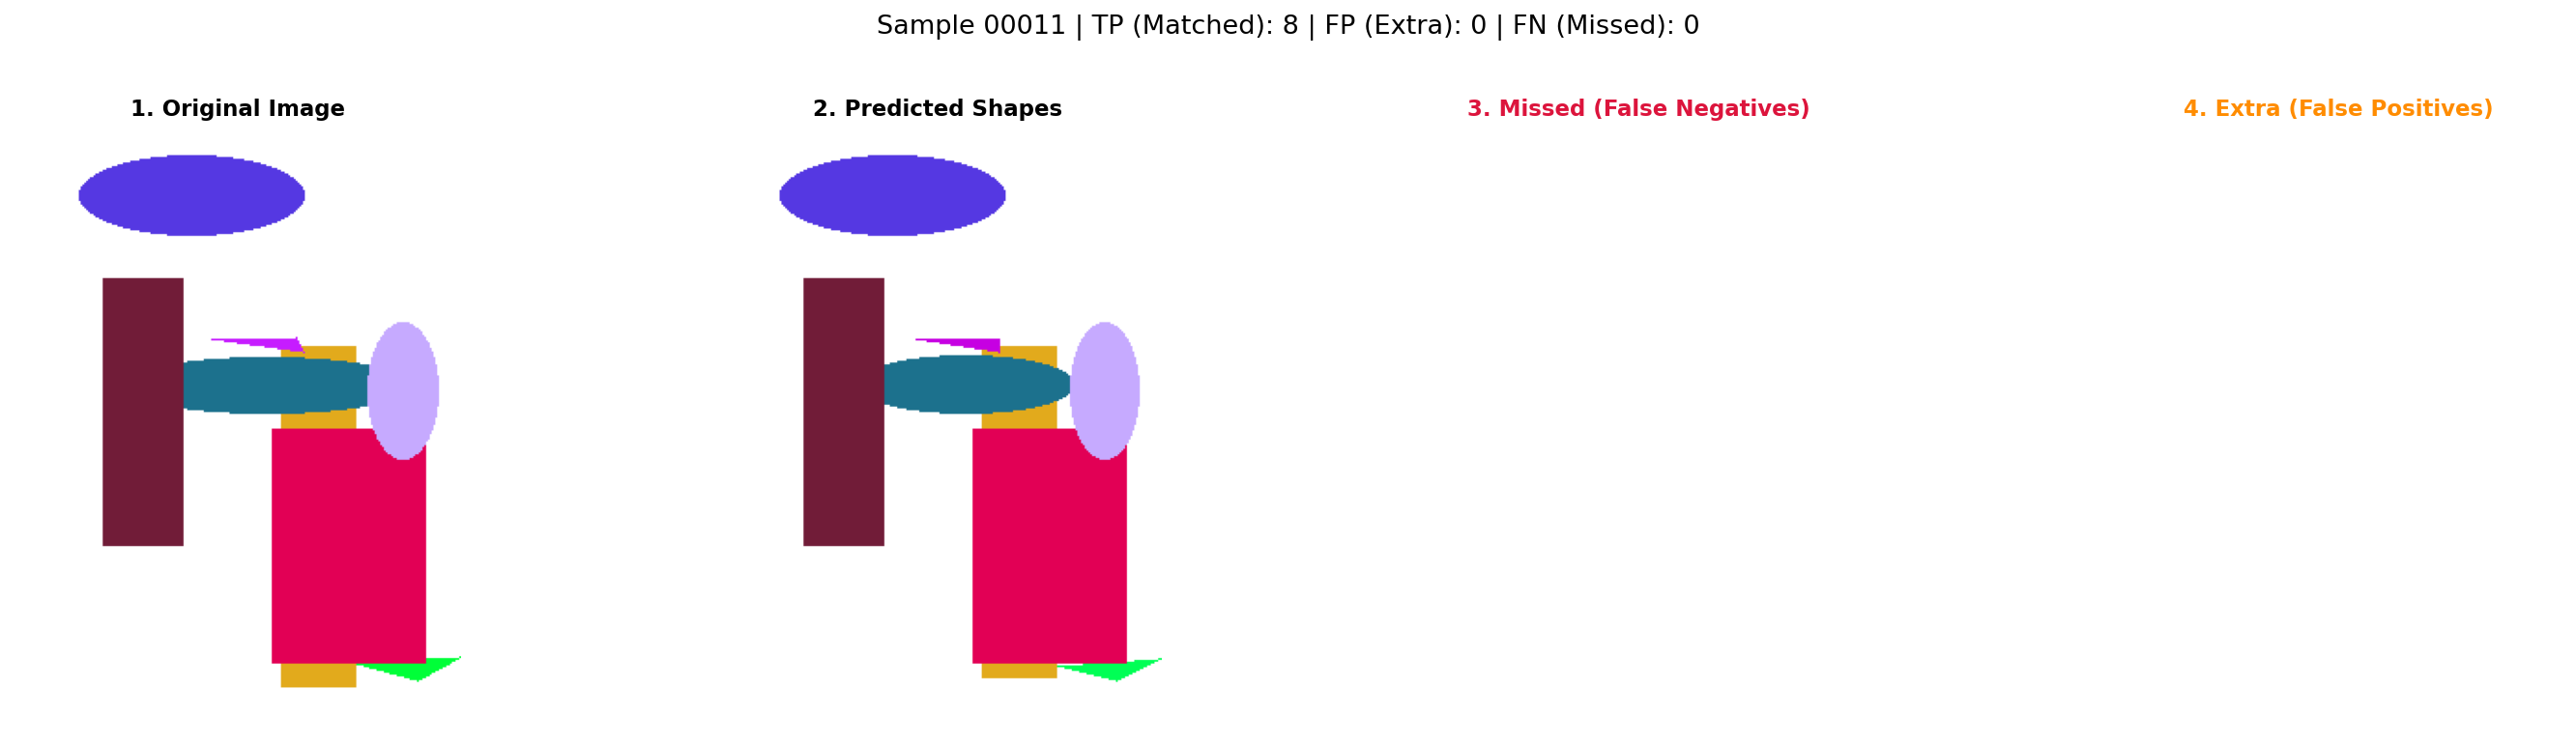
\includegraphics[width=\textwidth,keepaspectratio]{result}\\[0.15em]
{\small Пример~1 (9~фигур): TP\,=\,9, FP\,=\,0, FN\,=\,0}\\[0.6em]
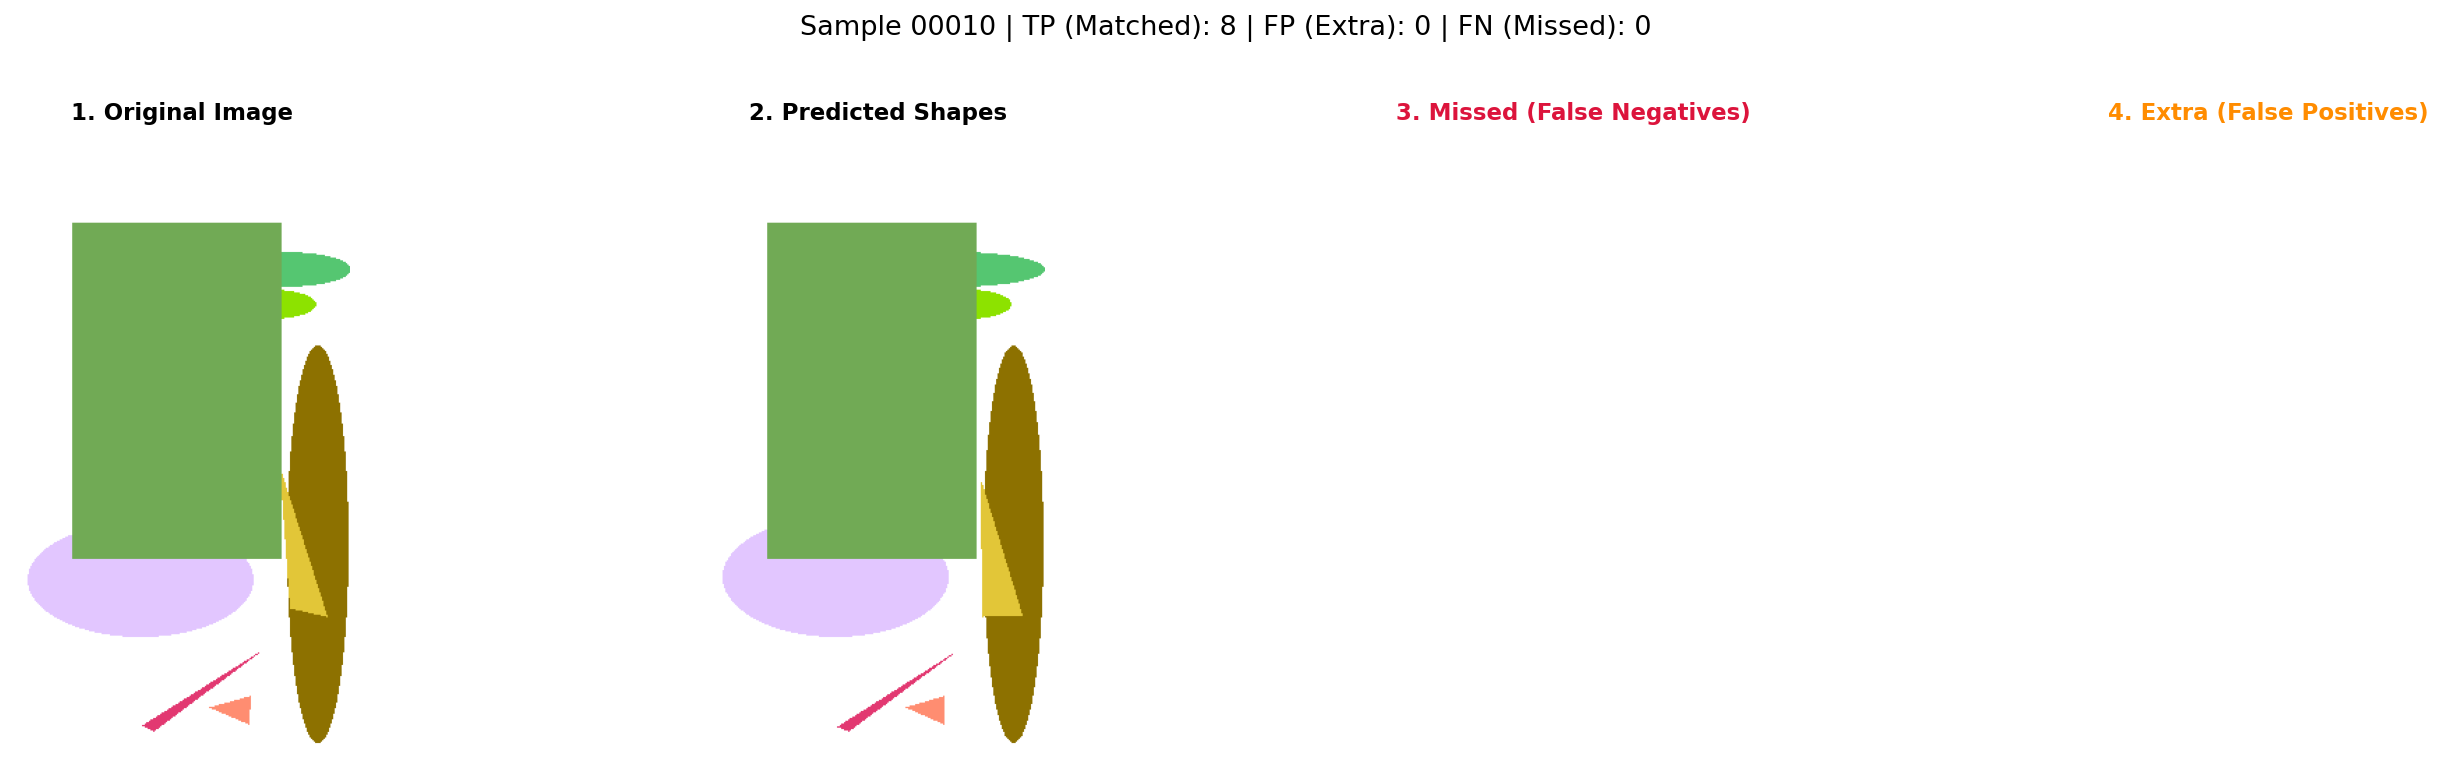
\includegraphics[width=\textwidth,keepaspectratio]{result2}\\[0.15em]
{\small Пример~2 (8~фигур): TP\,=\,8, FP\,=\,0, FN\,=\,0}
\end{center}
\end{frame}

\begin{frame}
\frametitle{Заключение}
\framesubtitle{Итоги и направления развития}
\textbf{Итоги:}
\begin{itemize}
  \item Реализована сквозная модель image-to-sequence, порождающая корректное JSON-описание сцены геометрических фигур.
  \item Двухэтапное обучение (MLE\,$+$\,RL) повышает геометрическое качество сверх посимвольного правдоподобия.
\end{itemize}
\textbf{Направления развития:}
\begin{itemize}
  \item Расширение набора типов фигур и~переход к~реальным изображениям.
  \item Учёт цвета и~порядка перекрытия (z-order) в~функции награды.
\end{itemize}
\end{frame}

\end{document}
